\newpage


\subsection{Schaltregler}
	\subsubsection{Grundprinzip}
		



\subsection{Abwärtswandler}
	\begin{minipage}{6cm}
		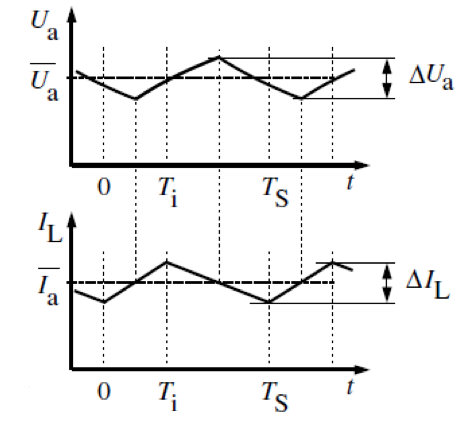
\includegraphics[width=4cm]{./images/schaltregler/06_buck-Verhalten}
	\end{minipage}
	\begin{minipage}{12cm}
		\begin{align*}
			&\text{Schalter geschlossen} & \Delta I_{L_{on}} &= \int_{0}^{T_i} (U_e - U_a) dt = \frac{1}{L} \cdot (U_e - U_a) \cdot T_i \\
			&\text{Schalter offen} & \Delta I_{L_{off}} &= \int_{T_i}^{T_s}(U_a + U_{F_0} dt = \frac{1}{L} \cdot (U_a - U_{F_0}) \cdot (T_s - T_i) \\
			&\text{Bilanz} & U_a &= \frac{T_i}{T_s} \cdot U_e - \left(1-\frac{T_i}{T_s} \right) \cdot U_{F_0} \approx \frac{T_i}{T_s} \cdot U_e
		\end{align*}
	\end{minipage}
	
\subsection{Invertierender Wandler}
	\begin{minipage}{6cm}
		\includegraphics[width=4cm]{./images/invWandler-Verhalten}
	\end{minipage}
	\begin{minipage}{12cm}
		\[ U_a = -\frac{T_i}{T_s} \cdot U_e \]
	\end{minipage}

\subsection{Ladungspumpen}
	Prinzip: Regelung der Ausgangsspannung durch Ändern der Schaltfrequenz \\
	\begin{minipage}{5cm}
		\includegraphics[width=4cm]{./images/ladungspumpe-normal}
	\end{minipage}
	\begin{minipage}{5cm}
		\includegraphics[width=4cm]{./images/ladungspumpe-inv}
	\end{minipage}
	\begin{minipage}{6cm}
		\begin{align*}
			\Delta U_a &= \frac{U_e - U_a}{1 + \frac{C_L}{C_1}} \\
			\Delta Q &= C_L \cdot \Delta U_a &= \frac{C_L \cdot C_1}{C_L + C_1} (U_e - U_a) \\
			I_a &= I_e = \frac{\Delta Q}{T_s} &= \frac{C_L \cdot C_1}{C_L + C_1} \frac{U_e - U_a}{T_s}
		\end{align*}
	\end{minipage}
	
\subsection{Effizienzsteigerung}
	\subsubsection{MOSFET statt Diode}
		\includegraphics[width=12cm]{images/effizient1}
		\begin{itemize}
		\begin{minipage}{8cm}
 		 	\item Diode hat Spannungsabfall
  			\begin{itemize}
    			\item Silizium-Diode: 0.7V
   				\item Schottky-Diode: 0.3V
    			\item MOSFET hat "`nur"' On-Widerstand $R_{DS_{on}}$
			\end{itemize}
		\end{minipage}
		\begin{minipage}{8cm}
			\item Umschalten vom Substratpotential beim Längstransistor nötig
   			\begin{itemize}
     			\item Synchronous rectifier
    		\end{itemize}
		\end{minipage}
		\end{itemize}